% \documentclass{article}

% \documentclass{book}

\documentclass{report}

\usepackage{contents/start/init}

\usepackage{contents/start/vvn}

\begin{document} % Bắt đầu

%%%%%%%%%%%%%%%%%%%%%%%%%%%%%%%%%%

% \begin{titlepage}

% Vẽ hình chữ nhật

\begin{tikzpicture}[remember picture, overlay]\draw [line width = 3pt]($ (current page.north west) + (3.0cm, - 2.5cm)$)rectangle($ (current page.south east) + (- 2.5cm, 2.5cm)$);\draw [line width = 0.5pt]($ (current page.north west) + (3.1cm, - 2.6cm)$)rectangle($ (current page.south east) + (- 2.6cm, 2.6cm)$);\end{tikzpicture}

\begin{center}

\vspace{- 0.4cm}

\textbf{ĐẠI HỌC BÁCH KHOA HÀ NỘI} \\

\textbf{VIỆN TOÁN ỨNG DỤNG VÀ TIN HỌC} \\

\textbf{******}

\vspace{0.8cm}

\begin{figure}[H]

\centering


\includegraphics[scale = 0.5]{pictures/hust/main.png}

\end{figure}

\vspace{0.7cm}

\textbf{\fontsize{16pt}{30pt}\selectfont {BÁO CÁO ĐỒ ÁN II}} \\

% \textbf{\fontsize{10pt}{24pt}\selectfont {Chuyên ngành: TOÁN TIN}}

\vspace{1cm}

\textbf{\fontsize{16pt}{30pt}\selectfont {ĐỀ TÀI:}} \\

\textbf{\fontsize{20pt}{24pt}\selectfont {Sử dụng thiết kế hướng miền \\ xây dựng kiến trúc vi dịch vụ cho \\ bài toán hóa đơn điện tử}} \\

\end{center}

\vspace{0.3cm}

% \begin{minipage}{0.8\textwidth}

\begin{center}

\textbf{\fontsize{10pt}{24pt}\selectfont {Chuyên ngành: Toán Tin}}

% \textbf{\fontsize{10pt}{24pt}\selectfont {Giảng viên hướng dẫn: TS. Vũ Thành Nam}}

\end{center}

% \end{minipage}

\vspace{0.7cm}

\hspace{3cm}\begin{minipage}{0.7\textwidth}

\begin{tabular}{l l l}

\textbf{\fontsize{10pt}{24pt}\selectfont {Giảng viên hướng dẫn}} & \textbf{\fontsize{10pt}{24pt}\selectfont {TS. Vũ Thành Nam}} \\

\textbf{\fontsize{10pt}{24pt}\selectfont {Sinh viên thực hiện}} & \textbf{\fontsize{10pt}{24pt}\selectfont {Vũ Văn Nghĩa}} \\

\textbf{\fontsize{10pt}{24pt}\selectfont {Mã số sinh viên}} & \textbf{\fontsize{10pt}{24pt}\selectfont {20206205}} \\

\textbf{\fontsize{10pt}{24pt}\selectfont {Lớp}} & \textbf{\fontsize{10pt}{24pt}\selectfont {Toán Tin 02 - K65}} \\

\end{tabular}

\end{minipage}

\vfill

\begin{center}

\textbf{Hà Nội, \the\year}

% \textbf{Hà Nội, \the\month~/~\the\year}

\end{center}

\end{titlepage}



% % Trang trắng không có nội dung và không có số trang

\pagestyle{empty}

\thispagestyle{empty}

\mbox{} % Một hộp rỗng để trang không bị trắng toàn bộ

\newpage



% \begin{titlepage}

% Vẽ hình chữ nhật

\begin{tikzpicture}[remember picture, overlay]\draw [line width = 3pt]($ (current page.north west) + (3.0cm, - 2.5cm)$)rectangle($ (current page.south east) + (- 2.5cm, 2.5cm)$);\draw [line width = 0.5pt]($ (current page.north west) + (3.1cm, - 2.6cm)$)rectangle($ (current page.south east) + (- 2.6cm, 2.6cm)$);\end{tikzpicture}

\begin{center}

\vspace{- 0.4cm}

\textbf{ĐẠI HỌC BÁCH KHOA HÀ NỘI} \\

\textbf{VIỆN TOÁN ỨNG DỤNG VÀ TIN HỌC} \\

\textbf{******}

\vspace{0.8cm}

\begin{figure}[H]

\centering


\includegraphics[scale = 0.5]{pictures/hust/main.png}

\end{figure}

\vspace{0.7cm}

\textbf{\fontsize{16pt}{30pt}\selectfont {BÁO CÁO ĐỒ ÁN II}} \\

% \textbf{\fontsize{10pt}{24pt}\selectfont {Chuyên ngành: TOÁN TIN}}

\vspace{1cm}

\textbf{\fontsize{16pt}{30pt}\selectfont {ĐỀ TÀI:}} \\

\textbf{\fontsize{20pt}{24pt}\selectfont {Sử dụng thiết kế hướng miền \\ xây dựng kiến trúc vi dịch vụ cho \\ bài toán hóa đơn điện tử}} \\

\end{center}

\vspace{0.3cm}

% \begin{minipage}{0.8\textwidth}

\begin{center}

\textbf{\fontsize{10pt}{24pt}\selectfont {Chuyên ngành: Toán Tin}}

% \textbf{\fontsize{10pt}{24pt}\selectfont {Giảng viên hướng dẫn: TS. Vũ Thành Nam}}

\end{center}

% \end{minipage}

\vspace{0.7cm}

\hspace{3cm}\begin{minipage}{0.7\textwidth}

\begin{tabular}{l l l}

\textbf{\fontsize{10pt}{24pt}\selectfont {Giảng viên hướng dẫn}} & \textbf{\fontsize{10pt}{24pt}\selectfont {TS. Vũ Thành Nam}} \\

\textbf{\fontsize{10pt}{24pt}\selectfont {Sinh viên thực hiện}} & \textbf{\fontsize{10pt}{24pt}\selectfont {Vũ Văn Nghĩa}} \\

\textbf{\fontsize{10pt}{24pt}\selectfont {Mã số sinh viên}} & \textbf{\fontsize{10pt}{24pt}\selectfont {20206205}} \\

\textbf{\fontsize{10pt}{24pt}\selectfont {Lớp}} & \textbf{\fontsize{10pt}{24pt}\selectfont {Toán Tin 02 - K65}} \\

\end{tabular}

\end{minipage}

\vfill

\begin{center}

\textbf{Hà Nội, \the\year}

% \textbf{Hà Nội, \the\month~/~\the\year}

\end{center}

\end{titlepage}



% % Trang trắng không có nội dung và không có số trang

\pagestyle{empty}

\thispagestyle{empty}

\mbox{} % Một hộp rỗng để trang không bị trắng toàn bộ

\newpage



% \newpage

\begin{center}

{\bfseries NHẬN XÉT CỦA GIẢNG VIÊN HƯỚNG DẪN}

\end{center}

\begin{enumerate}

\item Mục đích và nội dung của đồ án:

\vspace{20ex} % Thêm khoảng cách dọc

\item 	Kết quả đạt được:

\vspace{20ex} % Thêm khoảng cách dọc

\item 	Ý thức làm việc của sinh viên:

\vspace{20ex} % Thêm khoảng cách dọc

\end{enumerate}

\hspace{0.4\textwidth}\begin{minipage}{0.5\textwidth}

\noindent\begin{center}

\textit{Hà Nội, \today} \\

\textbf{Giảng viên hướng dẫn} \\

\textit{(Ký và ghi rõ họ tên)}

\vspace{2cm}

\textbf{TS. Vũ Thành Nam}

\end{center}

\end{minipage}

\pagestyle{empty}

\newpage



% 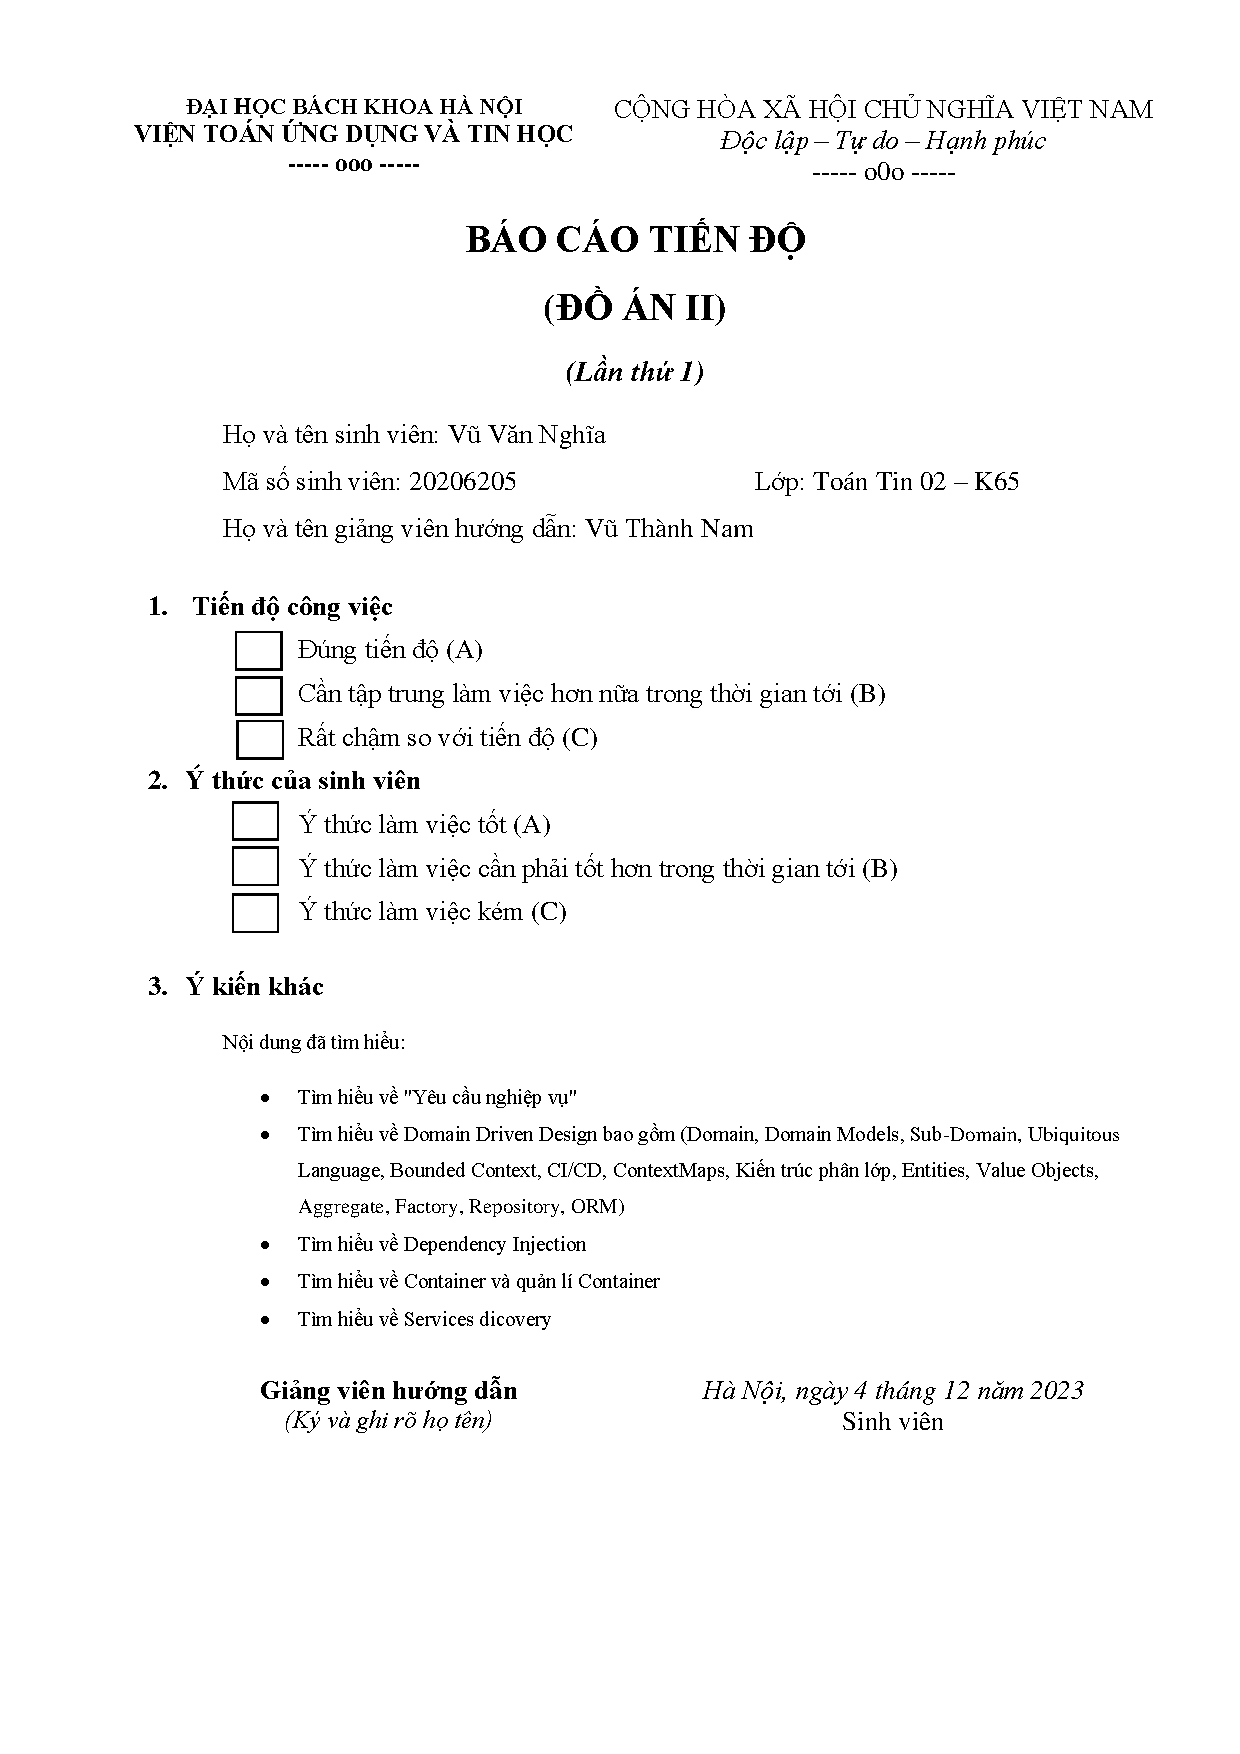
\includepdf[pages = -]{contents/chapter0/bao_cao_tien_do_1.pdf}

% 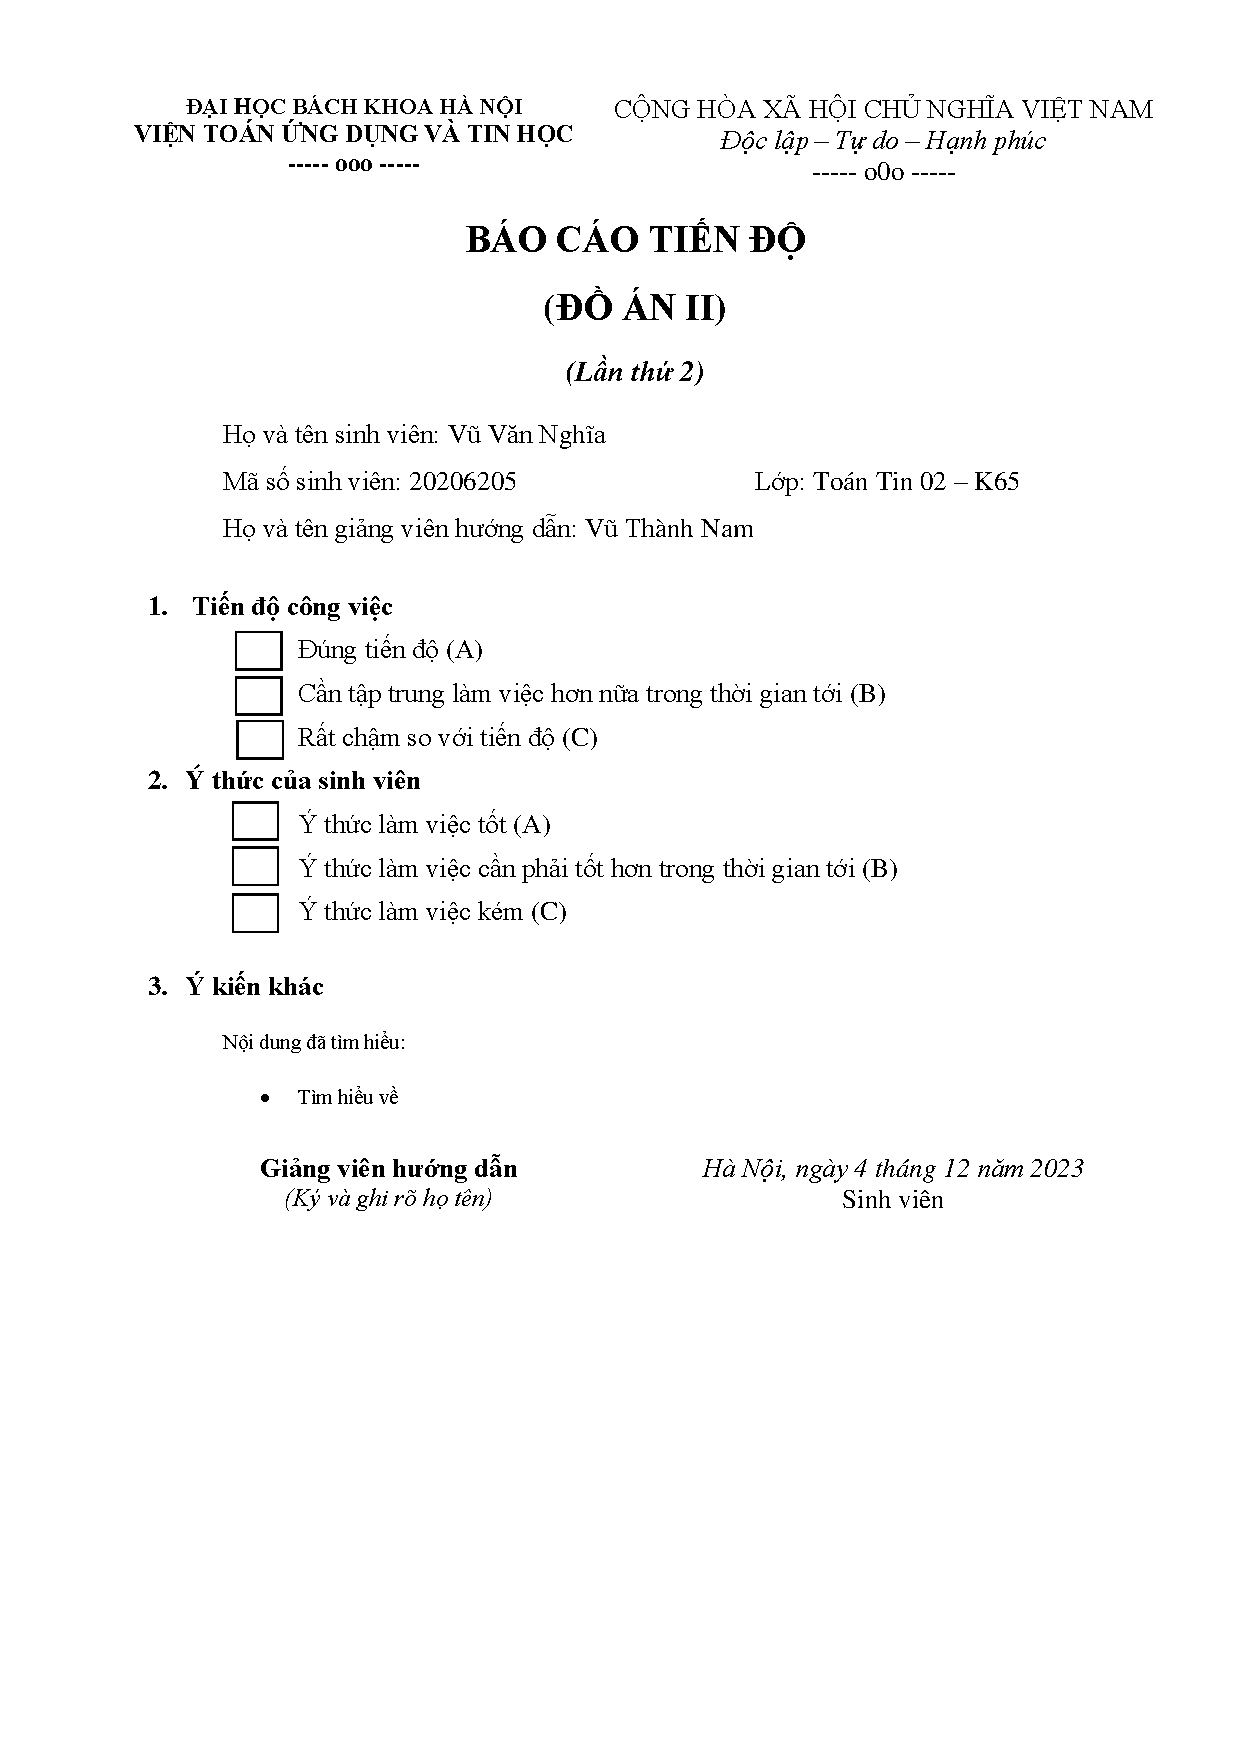
\includepdf[pages = -]{contents/chapter0/bao_cao_tien_do_2.pdf}

%%%%%%%%%%%%%%%%%%%%%%%%%%%%%%%%%%

% \newpage

\renewcommand*\contentsname{\centering MỤC LỤC}

\tableofcontents

\setcounter{page}{0}

% \newpage



%%%%%%%%%%%%%%%%%%%%%%%%%%%%%%%%%%

% \newpage

\chapter*{\centering LỜI CẢM ƠN}

\addcontentsline{toc}{chapter}{LỜI CẢM ƠN}

Trước hết, em xin gửi lời cảm ơn chân thành và sâu sắc của mình tới TS. Vũ Thành Nam, người thầy đã tận tình giúp đỡ và định hướng trong suốt thời gian thực hiện đồ án của em. Những kiến thức và kinh nghiệm mà em đã học được trong quá trình này sẽ giúp em phát triển và thành công trong tương lai. Em xin gửi lời chúc sức khỏe tới Thầy, mong rằng Thầy sẽ luôn dồi dào sức khỏe, đam mê và nhiệt huyết trong công việc giảng dạy.

Em cũng xin gửi lời cảm ơn tới các thầy cô giảng viên trong \textit{"Viện Toán ứng dụng và Tin học"} đã tận tình truyền đạt những kiến thức quý báu cho em. Những kiến thức này giúp em phát triển kiến thức, kỹ năng và lòng đam mê trong quá trình học tập, nghiên cứu.

\vspace{0.7cm}

\hspace{0.4\textwidth}\begin{minipage}{0.5\textwidth}

\noindent\begin{center}

\textit{Hà Nội, \today} \\

\textbf{Tác giả} \\

\textit{(Ký và ghi rõ họ tên)}

\vspace{2cm}

\textbf{Vũ Văn Nghĩa}

\end{center}

\end{minipage}

\newpage



% 

\chapter*{\centering DANH SÁCH BẢNG}

\addcontentsline{toc}{chapter}{DANH SÁCH BẢNG}

\makeatletter

\renewcommand\listoftables{

\@starttoc{lot}

}

\makeatother

\listoftables



% 

\chapter*{\centering DANH SÁCH HÌNH ẢNH}

\addcontentsline{toc}{chapter}{DANH SÁCH HÌNH ẢNH}

\makeatletter

\renewcommand\listoffigures{

\@starttoc{lof}

}

\makeatother

\listoffigures



% 

\chapter*{\centering DANH SÁCH CÁC CỤM TỪ VIẾT TẮT}

\addcontentsline{toc}{chapter}{DANH SÁCH CÁC CỤM TỪ VIẾT TẮT}

% @sau

\begin{table}[h]

\centering

\begin{tabular}{|c|c|c|c|}

\hline

STT & Từ viết tắt & Từ viết đầy đủ & Mô tả \\

\hline

Dong1 & Dong1 & Cot1 & Cot2 \\

\hline

Dong2 & Dong2 & Cot1 & Cot2 \\

\hline

\end{tabular}

\end{table}



% API; Application Programming Interface; Giao diện lập trình ứng dụng

% CI/CD; Continuous Integration (CI) and Continuous Delivery (CD) ; Quá trình tích hợp và chuyển giao liên tục

% thiết kế hướng miền ; thiết kế hướng miền; Kỹ thuật thiết kế theo hướng miền

% DI; Dependency Injection; Cơ chế tiêm sự phụ thuộc giữa các đối tượng

% HTTP; Hypertext Transfer Protocol; Giao thức truyền tải siêu văn bản

% JSON; JavaScript Object Notation; Một kiểu dữ liệu mở rộng của JavaScript

% ORM; Object Relational Mapping; Một kỹ thuật ánh xạ các đối tượng lập trình với từng bảng trong CSDL quan hệ

% Cơ sở dữ liệu ; CSDL ;

% Tạo (Create), Đọc (Read), Sửa (Update), Xóa (Delete) ; CRUD ;

% Kubernetes ; K8s ; kubernetes

% Số điện thoại ; SĐT ;

% UML

% MVC; Model View Controller; Một mẫu thiết kế ứng dụng

% SQL

SOA; Service Oriented Architecture; Kiến trúc hướng dịch vụ

SOAP; Simple Object Access Protocol; Một giao thức để truy cập dịch vụ web

SPA; Single Page Application; Kiểu ứng dụng một trang

REST; Representational State Transfer; Một tiêu chuẩn thiết kế các API sử dụng cho các dịch vụ web

URL; Uniform Resource Locator ; Địa chỉ định vị tài nguyên trên Internet

XML; Extensible Markup Language; Ngôn ngữ đánh dấu mở rộng

% TCT ; TCT ;

Người nộp thuế ; NNT ;

Mã số thuế ; MST ;

Hóa đơn điện tử ; HĐĐT ;

Cơ quan thuế ; CQT ;

Công nghệ thông tin ; CNTT ;



% \chapter*{\centering DANH SÁCH CÁC THUẬT NGỮ}

\addcontentsline{toc}{chapter}{DANH SÁCH CÁC THUẬT NGỮ}

% @sau

% @sau

\begin{table}[h]

\centering

\begin{tabular}{|c|c|c|}

\hline

STT & Tiếng Anh & Tiếng Việt \\

\hline

Dong1 & Dong1 & Cot2 \\

\hline

Dong2 & Dong2 & Cot2 \\

\hline

\end{tabular}

\end{table}

% kiến trúc nguyên khối, kiến trúc nguyên khối

% kiến trúc nguyên khối, kiến trúc nguyên khối

% kiến trúc vi dịch, kiến trúc vi dịch

% kiến trúc vi dịch, kiến trúc vi dịch

% kiến trúc vi dịch, kiến trúc vi dịch

% kiến trúc vi dịch, kiến trúc vi dịch

% thiết kế hướng miền, thiết kế hướng miền

% thiết kế hướng miền, thiết kế hướng miền

1 thiết kế hướng miền

Thiết kế hướng lĩnh vực

2 Domain (không dịch)

3 Abstraction Trừu tượng

4 chuyên gia ngành

\newpage

\chapter*{\centering MỞ ĐẦU}

\addcontentsline{toc}{chapter}{MỞ ĐẦU}

\section*{Lý do chọn đề tài}

Trong thời đại ngày nay, nhu cầu phát triển ứng dụng và hệ thống ngày càng tăng, đặt ra thách thức đối với kiến trúc phần mềm. Kiến trúc nguyên khối đã phục vụ hiệu quả trong quá khứ, nhưng kiến trúc này bắt đầu gặp khó khăn khi đối mặt với sự phức tạp, khả năng mở rộng và khả năng đáp ứng linh hoạt với sự thay đổi nhanh chóng trong yêu cầu kinh doanh.

Kiến trúc vi dịch vụ là giải pháp cho những thách thức trên. Kiến trúc vi dịch vụ chia dự án thành những dịch vụ nhỏ độc lập, mỗi dịch vụ chịu trách nhiệm về một chức năng cụ thể. Từ đó, dự án giảm sự phức tạp, tăng tính linh hoạt và dễ dàng quản lý.

Việc vận dụng kết hợp giữa kiến trúc vi dịch vụ và thiết kế hướng miền là một cách tiếp cận toàn diện, giúp xác định và tổ chức các dịch vụ dựa trên việc hiểu rõ về lĩnh vực kinh doanh. Thiết kế hướng miền xây dựng mô hình dựa trên yêu cầu nghiệp vụ thực tế, từ đó dự án phản ánh đúng các quy trình kinh doanh.

% Trong quá trình hoạt động kinh doanh, doanh nghiệp có nhu cầu chuyển đổi mô hình kinh doanh linh hoạt để có thể tồn tại và phát triển khi thị trường thay đổi. Từ đó, đáp ứng nhu cầu của khách hàng, mang lại ưu thế cạnh tranh so với các đối thủ.

Trong những năm gần đây, việc áp dụng kiến trúc vi dịch vụ ngày càng phổ biến, đem lại nhiều lợi ích như tách các nghiệp vụ kinh doanh thành các dịch vụ nhỏ độc lập, tăng tính linh hoạt và khả năng chống chịu sự cố.

Kiến trúc vi dịch vụ hỗ trợ doanh nghiệp chuyển đổi nhanh chóng để đáp ứng nhu cầu của mô hình kinh doanh và mong đợi của khách hàng. Tuy nhiên, để xây dựng được kiến trúc vi dịch vụ tốt, cần phải tạo ra các dịch vụ nhỏ phù hợp và duy trì tính độc lập. Trong đồ án này, em sử dụng thiết kế hướng miền để phân tích và xây dựng kiến trúc vi dịch vụ.

Theo quy định của Nghị định 123/2020/NĐ - CP, tất cả các doanh nghiệp, tổ chức và hộ kinh doanh đều bắt buộc phải sử dụng hóa điện tử. Vì vậy, nhu cầu sử dụng và xử lý hóa đơn điện tử trở nên rất lớn. Do đó trong đồ án này, em chọn chủ đề \emph{"Sử dụng thiết kế hướng miền xây dựng kiến trúc vi dịch vụ cho bài toán hóa đơn điện tử"}. Chủ đề này là một xu hướng quan trọng trong phát triển phần mềm và mang lại nhiều lợi ích trong việc cải thiện quá trình quản lý hóa đơn điện tử.



\end{document} % Kết thúc

% kết luận, tài liệu tham khảo

%%%%%%%%%%%%%%%%%%%%%%%%%%%%%%%%%%

\section*{Đối tượng và phạm vi nghiên cứu}

\begin{itemize}

\item \textbf{Đối tượng nghiên cứu:}

\item \textbf{Phạm vi nghiên cứu:}

\end{itemize}

\section*{Mot}

% ý nghĩa khoa học và thực tiễn của đề tài.

\subsection*{Đối tượng và phạm vi nghiên cứu}

\begin{itemize}

\item \textbf{Đối tượng nghiên cứu:} Hệ thống quản lí cửa hàng bán hàng.

\item \textbf{Phạm vi nghiên cứu:} Tập trung vào tìm hiểu kiến trúc kiến trúc vi dịch vụ và bước đầu xây dựng kiến trúc kiến trúc vi dịch vụ cho hệ thống quản lí cửa hàng bán hàng, bao gồm các thành phần như quản lý người dùng, quản lí sản phẩm, quản lí đơn hàng.

\end{itemize}

\subsection*{Ý nghĩa thực tiễn}

\begin{itemize}

\item \textbf{Dễ dàng mở rộng:} Kiến trúc kiến trúc vi dịch vụ cho phép mở rộng các phần tử của hệ thống một cách độc lập, giúp cửa hàng bán hàng mở rộng quy mô kinh doanh một cách linh hoạt và nhanh chóng.

\item \textbf{Dễ bảo trì:} Tách biệt các thành phần trong kiến trúc kiến trúc vi dịch vụ giúp giảm thiểu tác động của sự thay đổi lên các thành phần khác, làm cho quá trình bảo trì và cập nhật dễ dàng hơn.

\item \textbf{Tiết kiệm chi phí:} Hiệu quả hơn trong việc sử dụng tài nguyên hệ thống có thể giúp giảm thiểu chi phí vận hành và duy trì hệ thống.

\end{itemize}

%

\section*{Tóm tắt nội dung đồ án}

\addcontentsline{toc}{chapter}{Tóm tắt nội dung đồ án}

Báo cáo đồ án này sẽ được trình bày gồm 3 chương như sau:

\begin{itemize}

\item \textbf{Chương 1: Phân tích thiết kế hệ thống}

\begin{quote}

Nội dung phân tích hệ thống bán hàng.

\end{quote}

\item \textbf{Chương 2: Trình bày về kiến trúc kiến trúc vi dịch vụ}

\begin{quote}

Trình bày các công nghệ, kĩ thuật, nội dung của kiến trúc kiến trúc vi dịch vụ.

\end{quote}

\item \textbf{Chương 3: Các công nghệ đã sử dụng}

\begin{quote}

Trình bày các công nghệ em đã sử dụng trong đồ án này.

\end{quote}

\end{itemize}

Trong quá trình hoàn thành bài báo cáo này không tránh khỏi những thiếu sót. Vì vậy, em mong nhận được sự giúp đỡ và ý kiến đóng góp chân thành từ các thầy cô để em có thể cải thiện và hoàn thiện đề tài này một cách tốt nhất. Sự đóng góp quý báu của các thầy cô sẽ giúp em hiểu sâu hơn về đề tài và nắm vững hơn trong quá trình thực hiện.

\begin{flushleft}

\begin{adjustwidth}{0cm}{0cm}

Em xin chân thành cảm ơn!

\end{adjustwidth}

\begin{adjustwidth}{1cm}{0cm}

Sinh viên,

\end{adjustwidth}

\begin{adjustwidth}{0.8cm}{0cm}

Vũ Văn Nghĩa

\end{adjustwidth}

\end{flushleft}

% %%%%%%%%%%%%%%%%%%%%%%%%%%%%%%%%%%

% \chapter{Giới thiệu}

% \section{Mot}

% \subsection{Mot}

% \subsubsection{Mot}

% \begin{example} Bắt đầu

% \end{example}

%%%%%%%%%%%%%%%%%%%%%%%%%%%%%%%%%%

% Trong thời đại ngày nay, nhu cầu phát triển ứng dụng và hệ thống ngày càng tăng, đặt ra thách thức đối với kiến trúc phần mềm. Kiến trúc nguyên khối đã phục vụ hiệu quả trong quá khứ, nhưng kiến trúc này bắt đầu gặp khó khăn khi đối mặt với sự phức tạp, khả năng mở rộng và khả năng đáp ứng linh hoạt với sự thay đổi nhanh chóng trong yêu cầu kinh doanh.

Kiến trúc vi dịch vụ là giải pháp cho những thách thức trên. Kiến trúc vi dịch vụ chia dự án thành những dịch vụ nhỏ độc lập, mỗi dịch vụ chịu trách nhiệm về một chức năng cụ thể. Từ đó, dự án giảm sự phức tạp, tăng tính linh hoạt và dễ dàng quản lý.

Việc vận dụng kết hợp giữa kiến trúc vi dịch vụ và thiết kế hướng miền là một cách tiếp cận toàn diện, giúp xác định và tổ chức các dịch vụ dựa trên việc hiểu rõ về lĩnh vực kinh doanh. Thiết kế hướng miền xây dựng mô hình dựa trên yêu cầu nghiệp vụ thực tế, từ đó dự án phản ánh đúng các quy trình kinh doanh.

% \chapter{Giới thiệu}

% Trong thời đại ngày nay, nhu cầu phát triển ứng dụng và hệ thống ngày càng tăng, đặt ra thách thức đối với kiến trúc phần mềm. Kiến trúc nguyên khối đã phục vụ hiệu quả trong quá khứ, nhưng kiến trúc này bắt đầu gặp khó khăn khi đối mặt với sự phức tạp, khả năng mở rộng và khả năng đáp ứng linh hoạt với sự thay đổi nhanh chóng trong yêu cầu kinh doanh.

Kiến trúc vi dịch vụ là giải pháp cho những thách thức trên. Kiến trúc vi dịch vụ chia dự án thành những dịch vụ nhỏ độc lập, mỗi dịch vụ chịu trách nhiệm về một chức năng cụ thể. Từ đó, dự án giảm sự phức tạp, tăng tính linh hoạt và dễ dàng quản lý.

Việc vận dụng kết hợp giữa kiến trúc vi dịch vụ và thiết kế hướng miền là một cách tiếp cận toàn diện, giúp xác định và tổ chức các dịch vụ dựa trên việc hiểu rõ về lĩnh vực kinh doanh. Thiết kế hướng miền xây dựng mô hình dựa trên yêu cầu nghiệp vụ thực tế, từ đó dự án phản ánh đúng các quy trình kinh doanh.

% \section{Giới thiệu về bài toán hóa đơn điện tử}

% Bài toán hóa đơn điện tử là một phần quan trọng của quá trình chuyển đổi số. Trong quá khứ, mọi người thường sử dụng hóa đơn giấy truyền thống. Ngày nay, khi có quy định kế toán và quản lý tài chính, hóa đơn điện tử đã trở nên phổ biến giúp giảm bớt sự phụ thuộc vào giấy tờ. Cùng với sự phát triển của khoa học công nghệ đã giúp quản lý hiệu quả công việc và tối ưu hóa quy trình kế toán và tài chính.



% \emph{Theo em tìm hiểu có các khái niệm và căn cứ pháp lý liên quan sau đây:}

% \subsection{Hóa đơn}

% \emph{Theo quy định tại khoản 1 Điều 3 Nghị định 123/2020/NĐ - CP:}

% %%%%%%%%%%%%%%%%%%%%%%%%%%%%%%%%%%%%%!

Hóa đơn là chứng từ kế toán do tổ chức, cá nhân bán hàng hóa, cung cấp dịch vụ lập, ghi nhận thông tin bán hàng hóa, cung cấp dịch vụ. Hóa đơn được thể hiện theo hình thức hóa đơn điện tử hoặc hóa đơn do cơ quan thuế đặt in.

%%%%%%%%%%%%%%%%%%%%%%%%%%%%%%%%%%%%%!



% \subsection{Hóa đơn điện tử}

% \emph{Theo quy định tại khoản 2 Điều 3 Nghị định 123/2020/NĐ - CP:}

% %%%%%%%%%%%%%%%%%%%%%%%%%%%%%%%%%%%%%!

Hóa đơn điện tử là hóa đơn có mã hoặc không có mã của cơ quan thuế được thể hiện ở dạng dữ liệu điện tử do tổ chức, cá nhân bán hàng hóa, cung cấp dịch vụ lập bằng phương tiện điện tử để ghi nhận thông tin bán hàng hóa, cung cấp dịch vụ theo quy định của pháp luật về kế toán, pháp luật về thuế, bao gồm cả trường hợp hóa đơn được khởi tạo từ máy tính tiền có kết nối chuyển dữ liệu điện tử với cơ quan thuế, trong đó:

a. Hóa đơn điện tử có mã của cơ quan thuế là hóa đơn điện tử được cơ quan thuế cấp mã trước khi tổ chức, cá nhân bán hàng hóa, cung cấp dịch vụ gửi cho người mua. Mã của cơ quan thuế trên hóa đơn điện tử bao gồm số giao dịch là một dãy số duy nhất do hệ thống của cơ quan thuế tạo ra và một chuỗi ký tự được cơ quan thuế mã hóa dựa trên thông tin của người bán lập trên hóa đơn.

b. Hóa đơn điện tử không có mã của cơ quan thuế là hóa đơn điện tử do tổ chức bán hàng hóa, cung cấp dịch vụ gửi cho người mua không có mã của cơ quan thuế.

%%%%%%%%%%%%%%%%%%%%%%%%%%%%%%%%%%%%%!



% \subsection{Bắt buộc sử dụng hóa đơn điện tử từ 01/07/2022}

% \emph{Theo quy định tại khoản 1 Điều 59 Nghị định 123/2020/NĐ - CP:}

% %%%%%%%%%%%%%%%%%%%%%%%%%%%%%%%%%%%%%!

Nghị định này có hiệu lực thi hành kể từ ngày 01 tháng 7 năm 2022, khuyến khích cơ quan, tổ chức, cá nhân đáp ứng điều kiện về hạ tầng công nghệ thông tin áp dụng quy định về hóa đơn, chứng từ điện tử của Nghị định này trước ngày 01 tháng 7 năm 2022.

%%%%%%%%%%%%%%%%%%%%%%%%%%%%%%%%%%%%%!

% Chủ đề đồ án

$\Rightarrow$ Theo quy định, tất cả các doanh nghiệp, tổ chức và hộ kinh doanh đều bắt buộc phải chuyển từ sử dụng hóa đơn giấy sang hóa đơn điện tử bắt đầu từ tháng 07/2022. Vì vậy, nhu cầu sử dụng và xử lý hóa đơn điện tử trở nên rất lớn. Do đó ở đồ án này, em chọn chủ đề về quản lý hóa đơn điện tử.

% \subsection{Lưu trữ hóa đơn điện tử}

% \emph{Theo quy định tại khoản 1 Điều 11 Thông tư 32/2011/TT - BTC:}

%%%%%%%%%%%%%%%%%%%%%%%%%%%%%%%%%%%%%!

Người bán, người mua hàng hoá, dịch vụ sử dụng hóa đơn điện tử để ghi sổ kế toán, lập báo cáo tài chính phải lưu trữ hóa đơn điện tử theo thời hạn quy định của Luật Kế toán. Trường hợp hóa đơn điện tử được khởi tạo từ hệ thống của tổ chức trung gian cung cấp giải pháp hóa đơn điện tử thì tổ chức trung gian này cũng phải thực hiện lưu trữ hóa đơn điện tử theo thời hạn nêu trên.

%%%%%%%%%%%%%%%%%%%%%%%%%%%%%%%%%%%%%!

\emph{Theo quy định tại khoản 5 Điều 41 Luật số 88/2015/QH13:}

%%%%%%%%%%%%%%%%%%%%%%%%%%%%%%%%%%%%%!

1. Tài liệu kế toán phải được lưu trữ theo thời hạn sau đây:

a. Ít nhất là 05 năm đối với tài liệu kế toán dùng cho quản lý, điều hành của đơn vị kế toán, gồm cả chứng từ kế toán không sử dụng trực tiếp để ghi sổ kế toán và lập báo cáo tài chính.

b. Ít nhất là 10 năm đối với chứng từ kế toán sử dụng trực tiếp để ghi sổ kế toán và lập báo cáo tài chính, sổ kế toán và báo cáo tài chính năm, trừ trường hợp pháp luật có quy định khác.

c. Lưu trữ vĩnh viễn đối với tài liệu kế toán có tính sử liệu, có ý nghĩa quan trọng về kinh tế, an ninh, quốc phòng.

%%%%%%%%%%%%%%%%%%%%%%%%%%%%%%%%%%%%%!

% Thời gian lưu trữ

$\Rightarrow$ Như vậy, hóa đơn điện tử sẽ được lưu trữ trên hệ thống hóa đơn điện tử của nhà cung cấp hoặc doanh nghiệp với thời gian lưu trữ ít nhất là 10 năm theo quy định của pháp luật.



% \subsection{Một số lợi ích của hóa đơn điện tử}

% \emph{Một số lợi ích của hóa đơn điện tử:}

\begin{itemize}

\item Tuân thủ các quy định về thuế và pháp luật.

\item Thể hiện tính minh bạch: bảo vệ quyền lợi của người mua và người bán.

\item Giúp tiết kiệm chi phí in ấn, lưu trữ và bảo quản.

\item Loại bỏ rủi ro cháy, hỏng hoặc mất và dễ dàng sao lưu.

\item Dễ dàng tra cứu, phát hành, quản lý, tạo báo cáo và giảm thủ tục giấy tờ.

\item Giúp theo dõi tình hình tài chính của công ty (doanh thu, chi phí, lợi nhuận).

\end{itemize}



%%%%%%%%%%%%%%%%%%%%%%%%%%%%%%%%%%

% \section{Giới thiệu về kiến trúc vi dịch vụ}

% \subsection{Kiến trúc nguyên khối}

% Trước khi kiến trúc vi dịch vụ trở nên phổ biến, kiến trúc nguyên khối đã được áp dụng rộng rãi trong kiến trúc phần mềm truyền thống. Kiến trúc nguyên khối là kiến trúc phần mềm trong đó tất cả các thành phần của dự án được xây dựng thành một đơn vị triển khai duy nhất.

Trong kiến trúc nguyên khối, bất kỳ thay đổi nào đối với một thành phần đều yêu cầu toàn bộ dự án phải được kiểm thử và triển khai lại. Dẫn đến tốc độ phát triển chậm và thiếu khả năng mở rộng.

Ví dụ: Mô hình MVC (Model - View - Controller) là một trong những dạng của kiến trúc nguyên khối. Trong mô hình này, ứng dụng được chia thành ba thành phần chính:

\begin{itemize}

\item Mô hình (Model): Đại diện cho dữ liệu và logic xử lý dữ liệu.

\item Giao diện (View): Đại diện cho giao diện người dùng.

\item Bộ điều khiển (Controller): Nhận yêu cầu người dùng thông qua View, sau đó tương tác với Model để làm việc với dữ liệu.

\end{itemize}



% \subsection{Kiến trúc vi dịch vụ}

% Kiến trúc vi dịch vụ chia dự án thành các thành phần nhỏ hơn được gọi là các dịch vụ.

Mỗi dịch vụ tập trung vào một khả năng kinh doanh cụ thể.

Các dịch vụ độc lập và giao tiếp với nhau thông qua hạ tầng mạng.

Trong thực tế, nhiều dự án thường chuyển đổi một cách dần dần từ kiến trúc nguyên khối sang kiến trúc vi dịch vụ.

\begin{figure}[H]

% Khi nào Vẽ lại chất lượng cao hơn

\centering

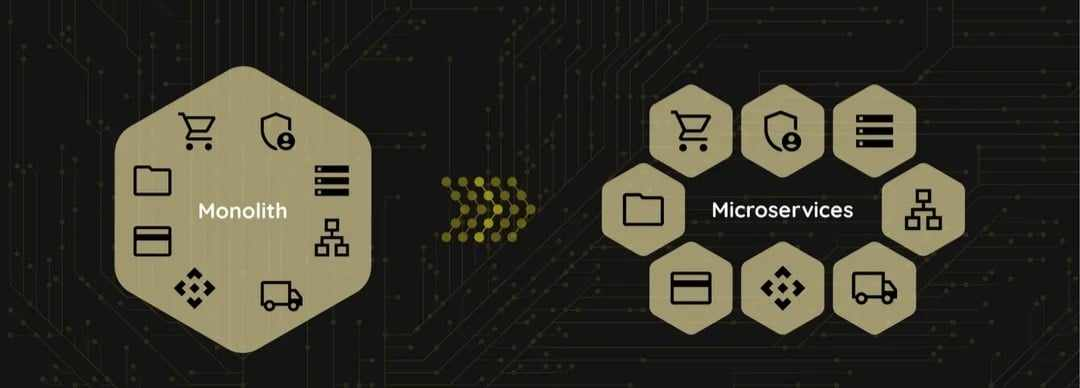
\includegraphics[scale = 0.4]{pictures/anh_khac_nhau_giua_kien_truc_nguyen_khoi_va_kien_truc_vi_dich_vu/main.jpg}

\caption{Ảnh khác nhau giữa kiến trúc nguyên khối và kiến trúc vi dịch vụ}

\end{figure}



% \subsection{Một số đặc điểm và ưu điểm của kiến trúc vi dịch vụ}

% Kiến trúc vi dịch vụ có nhiều ưu điểm, đặc biệt với các dự án có quy mô lớn và phức tạp.

\begin{itemize}

\item Kiến trúc vi dịch vụ phân chia dự án thành các dịch vụ nhỏ.

\begin{itemize}

\item Giúp việc phát triển và quản lý hệ thống dễ dàng hơn.

\item Tận dụng tài nguyên theo nhu cầu cho từng dịch vụ riêng.

\end{itemize}

\item Các dịch vụ độc lập về nghiệp vụ kinh doanh.

Các nhóm không cần hiểu sâu về mọi khía cạnh kinh doanh. Dẫn tới tốc độ phát triển và tốc độ định giá doanh nghiệp nhanh hơn.

\item Các dịch vụ độc lập về ngôn ngữ lập trình và CSDL

Ví dụ: Mỗi dịch vụ sử dụng ngôn ngữ lập trình và CSDL khác nhau như: NodeJS, Go, Python, Java, CSharp, MongoDB, SQLServer, SQLite, MySQL, PostgreSQL

\begin{figure}[H]

\centering

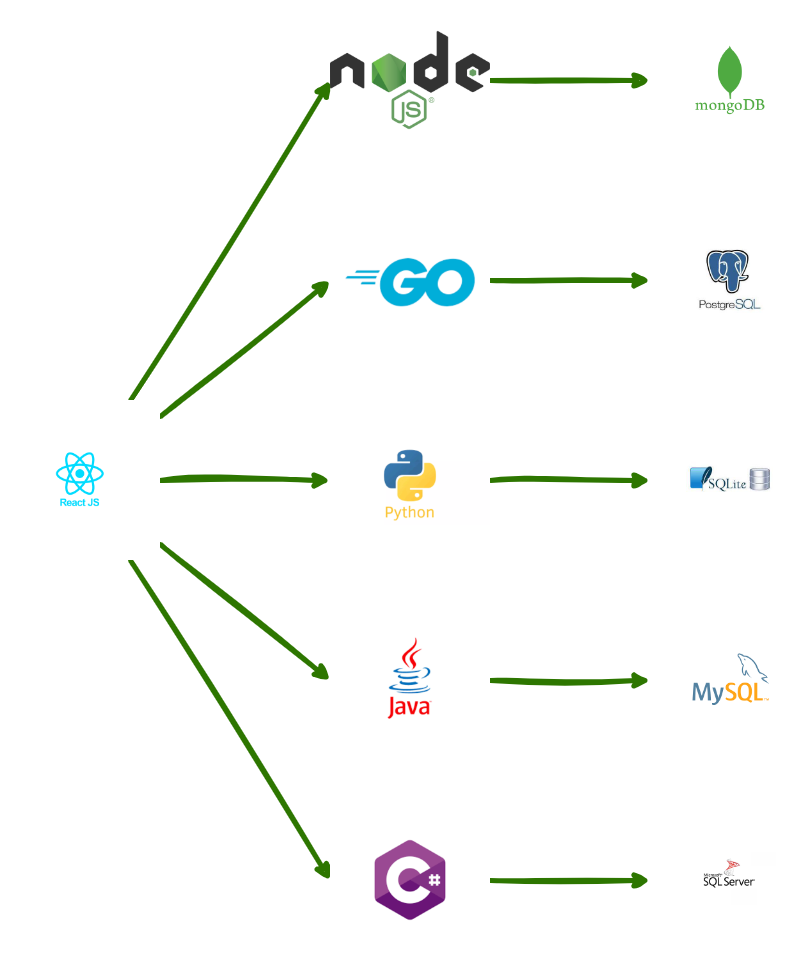
\includegraphics[scale = 0.3]{pictures/da_ngon_ngu_va_csdl/main.drawio.png}

\caption{Các dịch vụ độc lập về ngôn ngữ lập trình và CSDL}

\end{figure}

\begin{itemize}

\item Kiến trúc vi dịch vụ sử dụng đa ngôn ngữ và công nghệ khác nhau. Từ đó tận dụng hiệu quả thế mạnh của từng ngôn ngữ, công nghệ phù hợp nhất cho yêu cầu nghiệp vụ cụ thể.

\item Giảm chi phí và thời gian kiểm thử do ít ràng buộc.

\end{itemize}

\item Các dịch vụ độc lập về triển khai hệ thống

Mỗi dịch vụ triển khai độc lập và có thể thay đổi mà không ảnh hưởng đến các dịch vụ khác.

Giảm ràng buộc và tăng tính linh hoạt của hệ thống. Từ đó dễ dàng mở rộng hệ thống.

\item Hệ thống có khả năng chịu lỗi tăng độ tin cậy.

Do các dịch vụ độc lập, nhiều dịch vụ có thể triển khai trong cùng một khả năng kinh doanh để đảm bảo tính sẵn sàng của hệ thống.

\end{itemize}

%%%%%%%%%%%%%%%%%%%%%%%%%%%%%%%%%%%%%

% Các dịch vụ tương tác với nhau qua hạ tầng mạng.



% \newpage

% \subsection{Một số nhược điểm và thách thức của kiến trúc vi dịch vụ}

% Mặc dù kiến trúc vi dịch vụ có nhiều lợi ích, nhưng cũng có nhiều thách thức:

\begin{itemize}

\item Chịu ảnh hưởng của đường truyền mạng.

\item Đồng bộ đồng hồ thời gian.

\item Ràng buộc về thứ tự sự kiện.

\item Tính nhất quán và toàn vẹn của dữ liệu.

\item Khả năng kiểm soát giao dịch.

\item Giám sát giữa các dịch vụ.

\item Bảo mật giao tiếp giữa các dịch vụ.

\item Phát hiện lỗi và sửa lỗi khó khăn, phức tạp hơn.

\item Chi phí xây dựng và quản lý vận hành lớn.

\end{itemize}



%%%%%%%%%%%%%%%%%%%%%%%%%%%%%%%%%%

% \section{Giới thiệu về thiết kế hướng miền}

% Trong quá trình hoạt động kinh doanh, không phải mọi doanh nghiệp đều giữ nguyên mô hình kinh doanh được đưa ra ban đầu của mình. Khi quy mô thị trường thay đổi, việc chuyển đổi mô hình kinh doanh là điều cần thiết. Chuyển đổi kinh doanh như một công cụ linh hoạt giúp các doanh nghiệp có thể phát triển và tồn tại giữa các đối thủ của mình.

\begin{example}

\begin{itemize}

\item Google bắt đầu như công cụ tìm kiếm trực tuyến, nhưng sau đó đã mở rộng và thay đổi mô hình kinh doanh qua nhiều dịch vụ và sản phẩm khác nhau như: Dịch vụ đám mây Google Cloud Platform, Dịch vụ thư điện tử Gmail, Dịch vụ bản đồ Google Maps, Dịch vụ lưu trữ tập tin Google Drive, \dots

\item Amazon từ hiệu sách trực tuyến đã trở thành thị trường cho nhà cung cấp khác như: Thương mại điện tử, Dịch vụ đám mây Amazon Web Services (AWS), \dots

\begin{figure}[H]

\centering

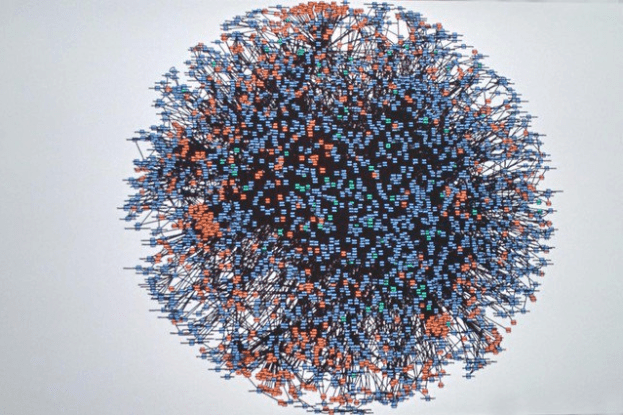
\includegraphics[scale = 0.5]{pictures/kien_truc_vi_dich_vu_cua_amazon/main.png}

\caption{Kiến trúc vi dịch vụ của Amazon}

\end{figure}

\end{itemize}

\end{example}

Đối với những doanh nghiệp không chuyển đổi kinh doanh sẽ không thể tồn tại.

\begin{example} Gần đây, dịch vụ giao đồ ăn Baemin đã rời khỏi thị trường Việt Nam cũng do sức ép từ các đối thủ khác khiến Baemin khó cạnh tranh trong mảng kinh doanh cốt lõi là giao đồ ăn. Các đối thủ này không chỉ cung cấp dịch vụ giao đồ ăn mà còn có đặt xe, giao hàng,...

\end{example}

\begin{figure}[H]

\centering

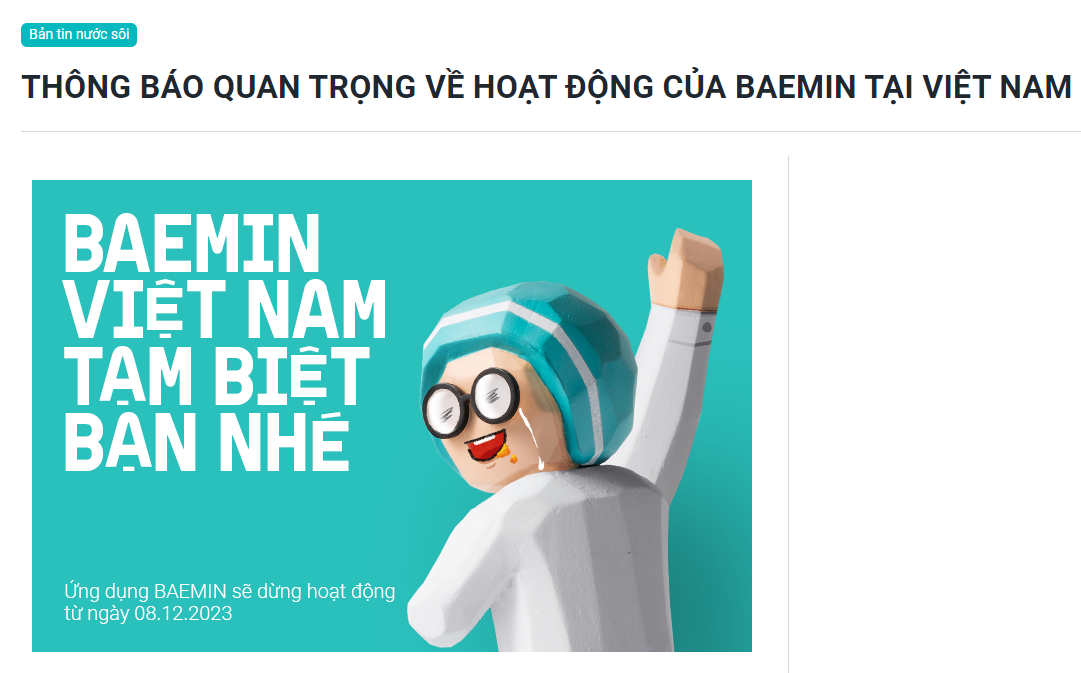
\includegraphics[scale = 0.5]{pictures/baemin/main.png}

\caption{Baemin đã rời khỏi thị trường Việt Nam}

\end{figure}

Hiện nay, các tổ chức doanh nghiệp có nhu cầu chuyển đổi kinh doanh để có thể tồn tại và phát triển khi thị trường thay đổi. Từ đó, đáp ứng nhu cầu của khách hàng, mang lại ưu thế cạnh tranh so với các đối thủ. Do đó, các doanh nghiệp cần hệ thống chuyển đổi nhanh chóng để đáp ứng nhu cầu của mô hình kinh doanh và mong đợi của khách hàng.

$\Rightarrow$ Kiến trúc vi dịch vụ giải quyết những thách thức và hỗ trợ doanh nghiệp chuyển đổi dễ dàng. Tuy nhiên, để xây dựng được kiến trúc vi dịch vụ tốt, cần phải tạo ra các dịch vụ nhỏ phù hợp và duy trì tính độc lập. Trong đồ án này, em sử dụng thiết kế hướng miền để phân tích và xây dựng kiến trúc vi dịch vụ. Thiết kế hướng miền xác định và tổ chức các dịch vụ dựa trên việc hiểu rõ về lĩnh vực kinh doanh, giúp dự án phản ánh đúng các quy trình và quy tắc kinh doanh.

%%%%%%%%%%%%%%%%%%%%%%%%%%%%%%%%%%%

%%%%%%%%%%%%%%%%%%%%%%%%%%%%%%%%%% @ \subsection{chưa xong}

% \chapter{Yêu cầu nghiệp vụ}

% \input{contents/yeu_cau_nghiep_vu}

% \subsection {Yêu cầu nghiệp vụ của bài toán phụ}

% \input{contents/yeu_cau_nghiep_vu_cua_bai_toan_phu}

% \subsubsection{Các chức năng tổng quan của bài toán phụ}

% \input{contents/cac_chuc_nang_tong_quan_cua_bai_toan_phu}

% \subsection{Yêu cầu nghiệp vụ chưa xong}

% \input{contents/yeu_cau_nghiep_vu_chua_xong}

%%%%%%%%%%%%%%%%%%%%%%%%%%%%%%%%%% @ \subsection{chưa xong}

%%%%%%%%%%%%%%%%%%%%%%%%%%%%%%%%%% @ \subsection{chưa xong}

%! chưa chắc vì mình có mẫu kt sẽ khác

%! chưa chắc vì mình có mẫu kt sẽ khác

% \chapter{Phân tích thiết kế hệ thống}

% \section{UML Use Case Diagrams}

% \section{UML Activity Diagrams}

% \section{UML Sequence Diagrams}

% \section{UML Class Diagrams}

%%%%%%%%%%%%%%%%%%%%%%%%%%%%%%%%%% @ \subsection{chưa xong}

%%%%%%%%%%%%%%%%%%%%%%%%%%%%%%%%%%

\chapter{Chi tiết và áp dụng thiết kế hướng miền}

\section{Đôi nét về thiết kế hướng miền (DomainDrivenDesign)}

Thiết kế hướng miền được Eric Evans giới thiệu trong cuốn sách "DomainDrivenDesign: Tackling Complexity in the Heart of Software".

Thiết kế hướng miền (DomainDrivenDesign) là một phương pháp thiết kế phần mềm tập trung vào việc hiểu rõ và mô hình hóa lĩnh vực kinh doanh của một tổ chức.

Thiết kế hướng miền nhấn mạnh việc sử dụng lĩnh vực nghiệp vụ kinh doanh để thảo luận và đề xuất giải pháp đáp ứng nhu cầu. Vì để tạo một phần mềm tốt, chúng ta cần phải hiểu rõ về chính phần mềm đó.

Trong nhiều ứng dụng thường có phần xử lý các công việc không liên quan đến vấn đề nghiệp vụ như truy cập file, hạ tầng mạng, CSDL,... trong đối tượng nghiệp vụ kinh doanh. Cách này giúp tốc độ hoàn thiện ứng dụng nhanh. Tuy nhiên, cách này làm cho thiết kế bị mất đi tính hướng đối tượng trong thực tế với mức độ doanh nghiệp lớn.

Trong kiến trúc vi dịch vụ, thiết kế hướng miền giúp đảm bảo rằng mỗi dịch vụ được thiết kế phản ánh một phần cụ thể của lĩnh vực kinh doanh. Mỗi dịch vụ được quản lí bởi một nhóm nhỏ được hỗ trợ bởi các chuyên gia ngành.



Trong thiết kế hướng miền, \emph{chuyên gia ngành (Domain Expert)} là người có kiến thức và hiểu biết sâu sắc về vấn đề đang được hệ thống phần mềm giải quyết. Chuyên gia ngành thể hiện chính xác vấn đề kinh doanh, đóng vai trò là nguồn thông tin cho nhóm phát triển.



\section{Định nghĩa miền (Domain)}

Hệ thống được tạo ra để xử lý sự phức tạp trong cuộc sống hiện đại. Việc phát triển hệ thống liên kết chặt chẽ với một số khía cạnh cụ thể trong cuộc sống của chúng ta.

Trong domain driven design, \emph{miền (Domain)} đề cập đến phạm vi kiến thức và vấn đề cụ thể mà hệ thống xử lý.

Xét theo góc độ kinh doanh và góc độ hệ thống:

\begin{itemize}

\item Về góc độ kinh doanh: miền đại diện cho một lĩnh vực hoặc ngành mà doanh nghiệp hoạt động.

\item Về góc độ hệ thống: miền có thể coi là đại diện cho không gian vấn đề của hệ thống.

\end{itemize}

Hệ thống cần phản ánh đúng miền và hiện thực hóa chính xác miền.

\begin{example} \emph{Trong đồ án này, miền được xác định là bài toán giải pháp hóa đơn điện tử.}

\end{example}

\section{Các mẫu trong thiết kế hướng miền}

Thiết kế hướng miền cung cấp 2 loại mẫu:

\begin{itemize}

\item \emph{Các mẫu chiến lược (Strategic Patterns):} Phân chia một miền lớn và phức tạp thành các phần nhỏ hơn với ranh giới được xác định rõ ràng. Giúp phân chia một miền lớn hợp lý.

\item \emph{Các mẫu kỹ thuật (Tactical Patterns):} Hiện thực hóa các khái niệm và qui trình trong thành phần thành các thiết kế hệ thống phần mềm. Giúp hệ thống phù hợp với kinh doanh.

\end{itemize}

\begin{figure}[H]

\centering

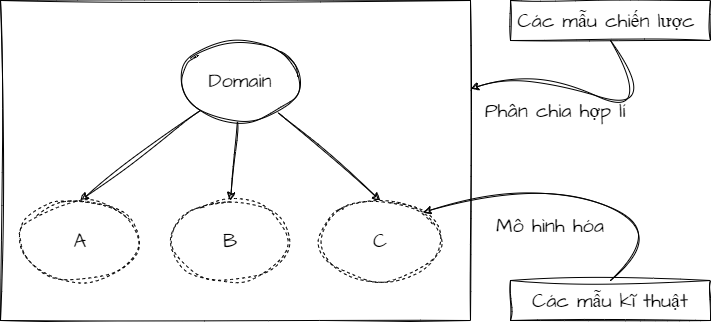
\includegraphics[scale = 0.5]{pictures/cac_mau_chien_luoc_va_cac_mau_ky_thuat/main.drawio.png}

\caption{Khái quát tổng quan về Strategic Patterns và Tactical Patterns}

\end{figure}

%%%%%%%%%%%%%%%%%%%%%%%%%%%%%%%%%%

\section{Các mẫu chiến lược}

\begin{itemize}

\item Các mẫu chiến lược phân tích nghiệp vụ kinh doanh sau đó đưa ra việc phân chia các thành phần và hiểu mối quan hệ của các thành phần đó.

\item Các mẫu chiến lược là giai đoạn xây dựng sự hiểu biết chung về miền giữa chuyên gia ngành và nhóm phân tích hệ thống.

\item Các mẫu chiến lược giúp xác định các thành phần quan trọng của hệ thống, đảm bảo kiến trúc phần mềm phản ánh đúng các yêu cầu kinh doanh.

$\Rightarrow$ Các mẫu chiến lược xác định mục tiêu tạo ra hệ thống có thể mở rộng, phát triển linh hoạt theo nhu cầu kinh doanh.

bao gồm:

\begin{itemize}

\item Muc1 %!nghia

\item Muc2 %!nghia

\item Muc1 %!nghia

\item Muc2 %!nghia

\item Muc1 %!nghia

\item Muc2 %!nghia

\item Muc1 %!nghia

\item Muc2 %!nghia

\end{itemize}

% nội dung trang lớn lên để hết giấy

\end{itemize}

\begin{figure}[H]

\centering

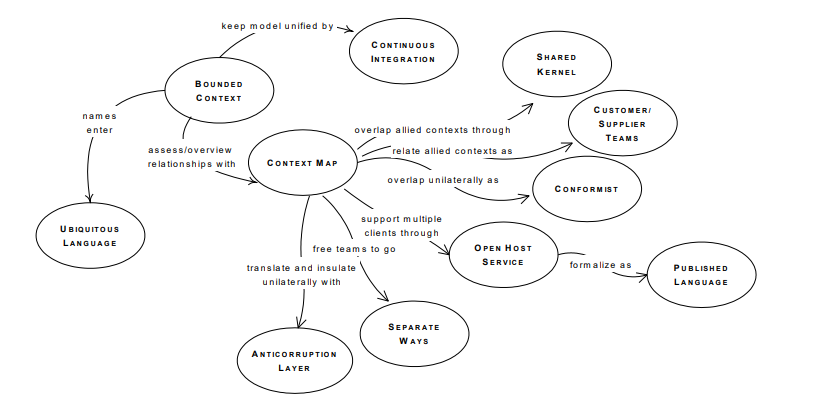
\includegraphics[scale = 0.9]{pictures/cac_mau_chien_luoc/temp.png}

\caption{Sơ đồ về các thành phần trong mô hình chiến lược}

\end{figure}

%!<! - - $ Vẽ lại sau: - - >

%!<! - - $ Vẽ lại sau: - - >

%!<! - - $ Vẽ lại sau: - - >

%!<! - - $ Vẽ lại sau: - - >

%!<! - - $ Vẽ lại sau: - - >

%!<! - - $ Vẽ lại sau: - - >

%!<! - - $ Vẽ lại sau: - - >

%!<! - - $ Vẽ lại sau: - - >

%!<! - - $ Vẽ lại sau: - - >

%!<! - - $ Vẽ lại sau: - - >



\newpage

\subsection{Miền phụ (Sub - Domain)}

Một miền lớn được tạo thành từ nhiều \emph{miền phụ (Sub - Domain)}. Trong thực tế, một miền kinh doanh phức tạp không thể có một chuyên gia ngành có kiến thức về tất cả các miền phụ.

\begin{example} Trong miền thương mại điện tử lớn có thể có một số miền phụ sau:

\begin{itemize}

\item \textbf{Miền phụ quản lý hàng tồn kho:} liên quan đến việc quản lý sản phẩm trong kho hàng.

\item \textbf{Miền phụ quản lý khách hàng:} liên quan đến việc quản lý tài khoản khách hàng.

\item \textbf{Miền phụ vận chuyển:} liên quan đến việc quản lý việc vận chuyển giao hàng.

\end{itemize}

\end{example}

% @Slide thì Phân loại các miền phụ

Trong thiết kế hướng miền, có ba loại miền phụ là:

\begin{itemize}

\item Miền phụ chung (Generic Subdomain)

\item Miền phụ cốt lõi (Core Subdomain)

\item Miền phụ hỗ trợ (Supporting Subdomain)

\end{itemize}

\subsubsection{Phân loại các miền phụ}

Trong thiết kế hướng miền, có ba loại miền phụ:

\begin{itemize}

\item Miền phụ chung (Generic Subdomain)

\item Miền phụ cốt lõi (Core Subdomain)

\item Miền phụ hỗ trợ (Supporting Subdomain)

\end{itemize}

\paragraph{Miền phụ chung (Generic Subdomain)}

\begin{itemize}

\item Miền phụ chung có thể được tìm thấy trên nhiều ngành.

\item Miền phụ chung cung cấp các giải pháp có sẵn mà doanh nghiệp có thể mua.

\item Doanh nghiệp không thể đạt được bất kỳ lợi thế cạnh tranh nào bằng cách thực hiện những điều khác biệt trong miền phụ chung.

\begin{example} Các miền phụ chung \textit{"quản lý nhân sự"} hay \textit{"quản lý cơ sở vật chất"} không tạo thêm bất kỳ giá trị khác biệt nào cho doanh nghiệp.

\end{example}

\end{itemize}

\paragraph{Miền phụ cốt lõi (Core Subdomain)}

\begin{itemize}

\item Miền phụ cốt lõi là điểm khác biệt quan trọng cho doanh nghiệp.

\item Miền phụ cốt lõi tập trung vào mục tiêu và yêu cầu của khách hàng với doanh nghiệp.

\item Miền phụ cốt lõi giúp phân biệt các doanh nghiệp và làm cho các doanh nghiệp có giá trị.

\item Miền phụ cốt lõi quyết định sự thành công của doanh nghiệp.

$\Rightarrow$ Vì vậy mỗi doanh nghiệp luôn tìm cách thực hiện những điều khác biệt trong các miền phụ cốt lõi này để đạt được một số lợi thế so với đối thủ cạnh tranh.

\begin{example} Trong miền thẻ tín dụng, miền phụ cốt lõi có thể là \textit{"phát hành thẻ"} chịu trách nhiệm về quá trình phát hành thẻ tín dụng cho khách hàng. Miền phụ cốt lõi này bao gồm các nhiệm vụ như: thu thập thông tin khách hàng, thực hiện kiểm tra tín dụng, kích hoạt thẻ, \dots

\end{example}

\end{itemize}



\paragraph{Miền phụ hỗ trợ (Supporting Subdomain)}

 Các miền phụ cốt lõi phụ thuộc vào các miền phụ hỗ trợ.         Miền phụ hỗ trợ cung cấp các dịch vụ để miền phụ cốt lõi hoạt động hiệu quả.     Tuy nhiên, miền phụ hỗ trợ không đòi hỏi mức độ phức tạp cao về logic nghiệp vụ.

\begin{example} Trong nhiều phần mềm, miền phụ hỗ trợ \textit{"xác thực người dùng"} OAuth 2.0 của Facebook hoặc Google hỗ trợ cho miền phụ cốt lõi hoạt động hiệu quả.

\end{example} 

\newpage

\subsubsection{Cách xác định các miền phụ}

Các miền phụ cốt lõi, hỗ trợ và chung có thể khác nhau đối với các doanh nghiệp hoạt động trong cùng một miền. Vì các miền phụ được xác định tùy theo nhu cầu kinh doanh và bối cảnh cụ thể của mỗi tổ chức.

\paragraph{Mô tả cách xác định các miền phụ}

\begin{enumerate}

\item Bắt đầu bằng cách xem xét nghiệp vụ kinh doanh.

\item Nếu có sẵn giải pháp đã biết thì có khả năng là miền phụ chung. Ngược lại, chúng ta kiểm tra nghiệp vụ kinh doanh đó có thêm giá trị kinh doanh nào hay không?

\item Nếu không có giá trị kinh doanh thì chúng ta kiểm tra xem các miền phụ cốt lõi có phụ thuộc vào miền phụ này hay không? Nếu có thì có khả năng là miền phụ hỗ trợ. Nếu không thì đó là miền phụ chung.

\item Nếu miền phụ có tiềm năng bổ sung một số giá trị kinh doanh thì bước kiểm tra tiếp theo là xem liệu miền doanh nghiệp có độ phức tạp cao hay không?

\item Nếu miền doanh nghiệp không có độ phức tạp cao thì có khả năng là miền phụ hỗ trợ. Ngược lại thì nó có khả năng là miền phụ cốt lõi.

\end{enumerate}

\begin{figure}[h]

\centering

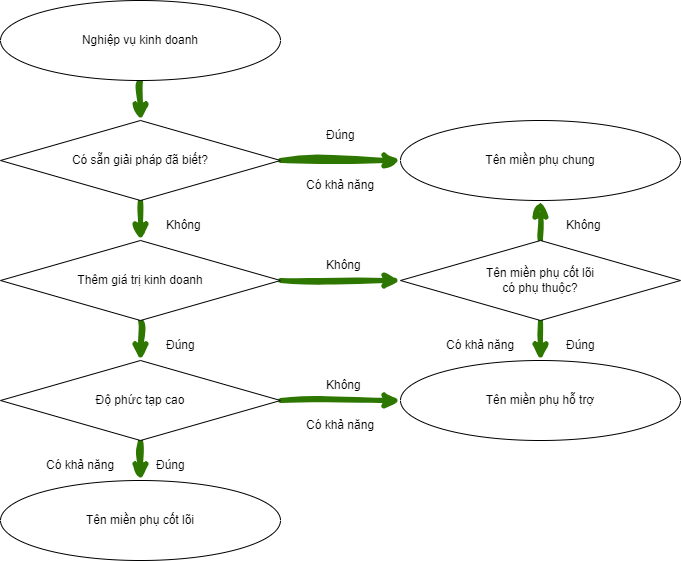
\includegraphics[scale = 0.5]{pictures/cach_xac_dinh_cac_mien_phu/main.drawio.png}

\caption{Sơ đồ xác định các miền phụ}

\end{figure}



\newpage

\subsubsection{Tại sao cần phân loại các miền phụ?}

Việc phân loại miền phụ giúp doanh nghiệp đưa ra quyết định với từng loại miền phụ khác nhau.

\begin{itemize}

\item Doanh nghiệp có nguồn lực hạn chế như nguồn nhân lực và kinh phí dành cho các sáng kiến. Việc phân loại các miền phụ giúp ưu tiên các sáng kiến khác nhau.

\item Các doanh nghiệp mong muốn tối đa hóa lợi nhuận đầu tư. Do đó, các sáng kiến liên quan đến miền phụ cốt lõi sẽ được ưu tiên.

\end{itemize}



\subsubsection{Áp dụng phân loại miền phụ trong đồ án này}

% %!<! - - Hướng dẫn: 5/3 - - >

% ChatGPT?

% Ứng dụng thiết kế hướng miền với hóa đơn điện tử thì miền phụ hỗ trợ có thể là gì?

\blindtext % Tạo văn bản ngẫu nhiên



\subsection{Mô hình miền (Domain Models)}

Để tạo một phần mềm tốt, chúng ta cần phải hiểu rõ về phần mềm đó. Trong thiết kế hướng miền để có thể hiểu miền nhanh, chúng ta cần tạo ra các mô hình miền.

Mô hình miền (Domain Models) là kiến thức có tổ chức và có cấu trúc về miền phù hợp để giải quyết vấn đề kinh doanh.

Mô hình miền không phải là kiến thức của chuyên gia ngành, mà là sự trừu tượng hóa của cả nhóm.

Trong quá trình phát triển, nhóm trao đổi và thảo luận về mô hình của nhóm.

Mô hình miền giúp nhóm hiểu công việc và đồng thuận khi làm việc.

Mục tiêu của mô hình miền là cung cấp rõ ràng, ngắn gọn và chính xác về miền làm cơ sở để hệ thống giải quyết vấn đề kinh doanh.

% @\begin{example} Trong đồ án này, mô hình miền của em bao gồm yêu câu nghiệp vụ và các sơ đồ: UML Use Case Diagrams, UML Activity Diagrams, UML Sequence Diagrams, UML Class Diagrams???????? \end{example}

\subsection{Bối cảnh giới hạn (Bounded Context)}

% \input{contents/boi_canh_gioi_han_bounded_context}

\subsection{Ngôn ngữ chung (Ubiquitous Language)}

% \input{contents/ngon_ngu_chung_ubiquitous_language}

\subsection{Bản đồ bối cảnh (Context Maps)}

% \input{contents/ban_do_boi_canh_context_maps}

\subsection{Chi tiết về các mối quan hệ bối cảnh giới hạn}

% \input{contents/chi_tiet_ve_cac_moi_quan_he_boi_canh_gioi_han}

\subsubsection{Mối quan hệ đối xứng (Symmetric Relationship)}

%%%%%%%%%%%%%%%%%%%%%%%%%%%%%%%%%%

\end{document} % Kết thúc

%%%%%%%%%%%%%%%%%%%%%%%%%%%%%%%%%%

%%%%%%%%%%%%%%%%%%%%%%%%%%%%%%%%%%

\subparagraph{Mô hình riêng biệt (Separate Ways)}

\input{contents/mo_hinh_rieng_biet_separate_ways}

\subparagraph{Mô hình hợp tác (Partnership)}

\input{contents/mo_hinh_hop_tac_partnership}

\subparagraph{Mô hình hạt nhân chung (Shared Kernel)}

\input{contents/mo_hinh_hat_nhan_chung_shared_kernel}

\end{document}

\paragraph{Mối quan hệ bất đối xứng (Asymmetric Relationship)}

\input{contents/moi_quan_he_bat_doi_xung_asymmetric_relationship}

\subparagraph{Mô hình khách hàng - nhà cung cấp (Customer - Supplier)}

\input{contents/mo_hinh_khach_hang_nha_cung_cap_customer_supplier}

\subparagraph{Mô hình tuân thủ (Conformist)}

\input{contents/mo_hinh_tuan_thu_conformist}

\subparagraph{Mô hình chống đổ vỡ (Anti Corruption Layer)}

\input{contents/mo_hinh_chong_do_vo_anti_corruption_layer}

\paragraph{Mối quan hệ 1 - nhiều (One to Many Relationship)}

\input{contents/moi_quan_he_1_nhieu_one_to_many_relationship}

\subparagraph{Dịch vụ máy chủ mở (Open Host Service)}

\input{contents/dich_vu_may_chu_mo_open_host_srv}

\subparagraph{Ngôn ngữ được xuất bản (Published Language)}

\input{contents/ngon_ngu_duoc_xuat_ban_published_language}

\subsection{Các mẫu kỹ thuật (Tactical Patterns)}

\end{document}

% Giới thiệu về Tactical Patterns

% \input{contents/cac_mau_ky_thuat_tactical}

\subsubsection{Các đối tượng miền (Domain Object)}

% \input{contents/cac_doi_tuong_mien_domain_object}

\paragraph{Đối tượng thực thể (Entities Objects)}

% \input{contents/doi_tuong_thuc_the_entities_objects}

\paragraph{Đối tượng giá trị (Value Objects)}

% \input{contents/doi_tuong_gia_tri_value_objects}

\paragraph{Miền dịch vụ (Service)}

% \input{contents/mien_dich_vu_srv}

% %! Hướng dẫn 7/4

% %! Hướng dẫn 7/5

% \subsubsection{xxxxxxx}

% Trong thời đại ngày nay, nhu cầu phát triển ứng dụng và hệ thống ngày càng tăng, đặt ra thách thức đối với kiến trúc phần mềm. Kiến trúc nguyên khối đã phục vụ hiệu quả trong quá khứ, nhưng kiến trúc này bắt đầu gặp khó khăn khi đối mặt với sự phức tạp, khả năng mở rộng và khả năng đáp ứng linh hoạt với sự thay đổi nhanh chóng trong yêu cầu kinh doanh.

Kiến trúc vi dịch vụ là giải pháp cho những thách thức trên. Kiến trúc vi dịch vụ chia dự án thành những dịch vụ nhỏ độc lập, mỗi dịch vụ chịu trách nhiệm về một chức năng cụ thể. Từ đó, dự án giảm sự phức tạp, tăng tính linh hoạt và dễ dàng quản lý.

Việc vận dụng kết hợp giữa kiến trúc vi dịch vụ và thiết kế hướng miền là một cách tiếp cận toàn diện, giúp xác định và tổ chức các dịch vụ dựa trên việc hiểu rõ về lĩnh vực kinh doanh. Thiết kế hướng miền xây dựng mô hình dựa trên yêu cầu nghiệp vụ thực tế, từ đó dự án phản ánh đúng các quy trình kinh doanh.

\end{document} % kết thúc

paragraph

% %

% % %! Aggregates/ /

% % Tổng hợp là đối tượng kinh doanh trung tâm trong Bối cảnh giới hạn của chúng ta và xác định phạm vi nhất quán trong bối cảnh giới hạn đó.

% % Tổng hợp = Mã định danh chính của Bối cảnh giới hạn của chúng ta

% \subsubsection{xxxxxxx}

% % Trong thời đại ngày nay, nhu cầu phát triển ứng dụng và hệ thống ngày càng tăng, đặt ra thách thức đối với kiến trúc phần mềm. Kiến trúc nguyên khối đã phục vụ hiệu quả trong quá khứ, nhưng kiến trúc này bắt đầu gặp khó khăn khi đối mặt với sự phức tạp, khả năng mở rộng và khả năng đáp ứng linh hoạt với sự thay đổi nhanh chóng trong yêu cầu kinh doanh.

Kiến trúc vi dịch vụ là giải pháp cho những thách thức trên. Kiến trúc vi dịch vụ chia dự án thành những dịch vụ nhỏ độc lập, mỗi dịch vụ chịu trách nhiệm về một chức năng cụ thể. Từ đó, dự án giảm sự phức tạp, tăng tính linh hoạt và dễ dàng quản lý.

Việc vận dụng kết hợp giữa kiến trúc vi dịch vụ và thiết kế hướng miền là một cách tiếp cận toàn diện, giúp xác định và tổ chức các dịch vụ dựa trên việc hiểu rõ về lĩnh vực kinh doanh. Thiết kế hướng miền xây dựng mô hình dựa trên yêu cầu nghiệp vụ thực tế, từ đó dự án phản ánh đúng các quy trình kinh doanh.

% \end{document} % kết thúc

% Yêu cầu nghiệp vụ của từng sub

% %

% Sơ đồ if else Đ S

% %

% sub trước model

% %

%%%%%%%%%%%%%%%%%%%%%%%%%%%%%%%%%%%%%

\end{document}

\section{xxxxxxx}

\subsection{xxxxxxx}

\subsubsection{xxxxxxx}

Trong thời đại ngày nay, nhu cầu phát triển ứng dụng và hệ thống ngày càng tăng, đặt ra thách thức đối với kiến trúc phần mềm. Kiến trúc nguyên khối đã phục vụ hiệu quả trong quá khứ, nhưng kiến trúc này bắt đầu gặp khó khăn khi đối mặt với sự phức tạp, khả năng mở rộng và khả năng đáp ứng linh hoạt với sự thay đổi nhanh chóng trong yêu cầu kinh doanh.

Kiến trúc vi dịch vụ là giải pháp cho những thách thức trên. Kiến trúc vi dịch vụ chia dự án thành những dịch vụ nhỏ độc lập, mỗi dịch vụ chịu trách nhiệm về một chức năng cụ thể. Từ đó, dự án giảm sự phức tạp, tăng tính linh hoạt và dễ dàng quản lý.

Việc vận dụng kết hợp giữa kiến trúc vi dịch vụ và thiết kế hướng miền là một cách tiếp cận toàn diện, giúp xác định và tổ chức các dịch vụ dựa trên việc hiểu rõ về lĩnh vực kinh doanh. Thiết kế hướng miền xây dựng mô hình dựa trên yêu cầu nghiệp vụ thực tế, từ đó dự án phản ánh đúng các quy trình kinh doanh.

% phải có CQRS (Phân chia trách nhiệm truy vấn lệnh)

CQRS là một mẫu kiến trúc riêng biệt có thể được sử dụng kết hợp với thiết kế hướng miền để đạt được những lợi ích nhất định, chẳng hạn như cải thiện hiệu suất và khả năng mở rộng. Tuy nhiên, nó không phải là một yêu cầu để triển khai thiết kế hướng miền.

% phải có event

Ngôn ngữ chung (Ubiquitous Language)

%%%%%%%%%%%%%%%%%%%%%%%%%%%%%%%%%%%%%

\end{document} % kết thúc

Cách tiếp cận này nhấn mạnh tính mô - đun, tính linh hoạt và khả năng phục hồi, cho phép các nhóm làm việc đồng thời trên các phần khác nhau của hệ thống và cho phép phát hành nhanh hơn và thường xuyên hơn. Các vi dịch vụ thường dựa vào các giao thức truyền thông nhẹ, chẳng hạn như REST và thường được triển khai bằng các công nghệ chứa trong bộ chứa như Docker và Kubernetes.

\subsubsection{DevOps Ứng dụng, áp dụng, liên quan,....}

\subsubsection{CI/CD}

\subsubsection{Docker}

\subsubsection{Kubernetes}

%@ Tất cả phải dùng ulli